The following aspects of the application are to be tested in order to help determine whether Google Glass is a viable option to use as replacement for an instruction manual when assembling components. Each test will be performed 30 times, for statistical significance~\cite{30sampleSize}.

\subsubsection{Text Length}
Since the Google Glass display is small and limited in space, the amount of text that may by displayed on screen is as a result also limited. As such, one interesting test case is to see where the text limit lies. The test consists of trying to find the text length limit, on both the Google Glass display, as well as a smartphone display. The text used should consist of characters distributed in similar fashion to English text~\cite{englishTextStat}.

When the smartphone display has been filled with information, how many slides does the same amount of information require on Google Glass? If the number of slides that the Google Glass application must use in order to display all the information is significantly greater than that of the smartphone application, the use of a Google Glass application might not be preferred as the user must potentially scroll through more slides than when using a smartphone equivalent application.

%\subsubsection{Tap Counter}


\subsubsection{Distance to the QR Code}
Generally, the recommendation regarding at what distance the user should be positioned, in relation to the QR code, is the size of the QR code times ten~\cite{qrCodeSizeComplexity}. However, different devices will have different delay time before registering the QR code in frame. As such, one test regards the time from the start of the camera until Google Glass has registered the QR code. The time is to be compared with that of smartphones.

%Table~\ref{tab:distanceAverage} shows how the results will be presented. 
Three different distances will be tested. The size of the QR code will be optimised according to the formula stated above, with the scanning distance set at two decimeters. The reason for testing for other scanning distances, yet with the same QR code size is because most users might not be aware of the optimal scanning distance, as well as to determine whether Google Glass has any advantages when scanning either closer to or further away from the QR code.

The size of the QR code is calculated as \[\frac{2}{10} = 0.2~decimeters\].
%SCALING FACTOR:
% http://www.growthvine.com/blogs/kelly-flowers/2011/11/28/optimal-size-for-qr-codes-depend-on-a-few-things

%	\begin{table}[ht!]
%    		\caption{Average time of registering a QR code with varying distances.} \label{tab:distanceAverage}
%		\centering \begin{tabularx}{\textwidth}{l|X|X|X} \hline
%		\textbf{Distance (dm)} & \textbf{Google Glass (ms)} & \textbf{Samsung Galaxy SII (ms)} & \textbf{Samsung Galaxy SIII (ms)} \\ \hline \hline
       
%		1.0	&	&	&	\\ \hline
%		2.0	&	&	&	\\ \hline
%		3.0	&	&	&	\\ \hline
		
%		\end{tabularx}
%	\end{table}

\subsubsection{Complexity of the QR Code}
Depending on the number of characters encoded by the QR code, the density of the QR code changes. The density of the QR code increases as the number of characters encoded by the QR code increases. In other words, the number of black and white squares increase. As such, one interesting test case is where the variable is the density of the QR code, or more specific; the number of characters encoded in the QR code.

The number of characters will vary between 1, 50 and 100. The values were chosen in order to give the results big enough room so that potential difference can be determined while still keeping the number of characters to a realistic minimum. %Table~\ref{tab:complexityAverage} shows how the results will be presented, where the results will be the average of 30 test runs.

%	\begin{table}[ht!]
%    		\caption{Average time of registering a QR code with varying density.} \label{tab:complexityAverage}
%		\centering \begin{tabularx}{\textwidth}{l|X|X|X} \hline
%		\textbf{Encoded Characters} & \textbf{Google Glass (ms)} & \textbf{Samsung Galaxy SII (ms)} & \textbf{Samsung Galaxy SIII (ms)} \\ \hline \hline
       
%		1	&	&	&	\\ \hline
%		50	&	&	&	\\ \hline
%		100	&	&	&	\\ \hline
		
%		\end{tabularx}
%	\end{table}

\subsubsection{Display Time}
The speed at which Google Glass registers the QR code is important to whether the device will gain preference over regular smartphones. However, another interesting aspect is how fast downloaded information may be displayed on screen, from the point that the information has been downloaded. %As seen in Table~\ref{tab:averageDisplaySpeedGoogleGlass}, which shows how the results will be presented, 
This test will evaluate three different information sizes, meant to represent three different ways of presenting information. 100 kilobyte represent text, 1 megabyte represent an image and 10 megabyte represent video.

%	\begin{table}[ht!]
%  		\caption{Average display time for Google Glass with varying information size.} \label{tab:averageDisplaySpeedGoogleGlass}
%		\centering \begin{tabularx}{\textwidth}{l|X|X|X} \hline
%		\textbf{Information Size (Byte)} & \textbf{Google Glass (ms)}  & \textbf{Samsung Galaxy SII (ms)}  & \textbf{Samsung Galaxy SIII (ms)} \\ \hline \hline
       
%		100 k	&	&	&	 \\ \hline
%		1 M		&	&	&	 \\ \hline
%		10 M		&	&	&	 \\ \hline

%		\end{tabularx}
%	\end{table}

%\subsection{Number of Tests}
%Only looking at the three last test cases the number of tests that must be performed are 30 for each different varying factor, on three different devices. The number of tests can as such be calculated as follows:
%
%\[30 * 3 * 3 * 3 = 810~tests\]
%
%However, since some of the tests will overlap in terms of their set-up the number of tests can be reduced as described in Figure~\ref{testCombination}, giving the following number of tests:
%
%\[30 * 7 * 3 = 630~tests\]
%
%The number of tests may be reduced this way as the distance between the QR code and the specific device in the complexity test and the display time test will be 2 decimeters. The complexity used for the distance test and the display time test will be that of one character, as the ID connected to the database is only one character (one identifying number, to be more specific). The display time will, however, have no effect on neither the distance test or the complexity test as the distance test and the complexity test and done prior to the information being downloaded from the back-end, in contrast the the display time which will be calculated after the information has been downloaded from the back-end.
%
%Looking at Figure~\ref{projectmap} the distance test and the complexity test will cover step 1 and 2 in the application, and the display time test will cover step 4. Step 3 is part of the back-end and as such not dependent on the device used, which is why step 3 will not be tested.
%
%	\begin{figure}[H]%ht!]
%		\centering
%		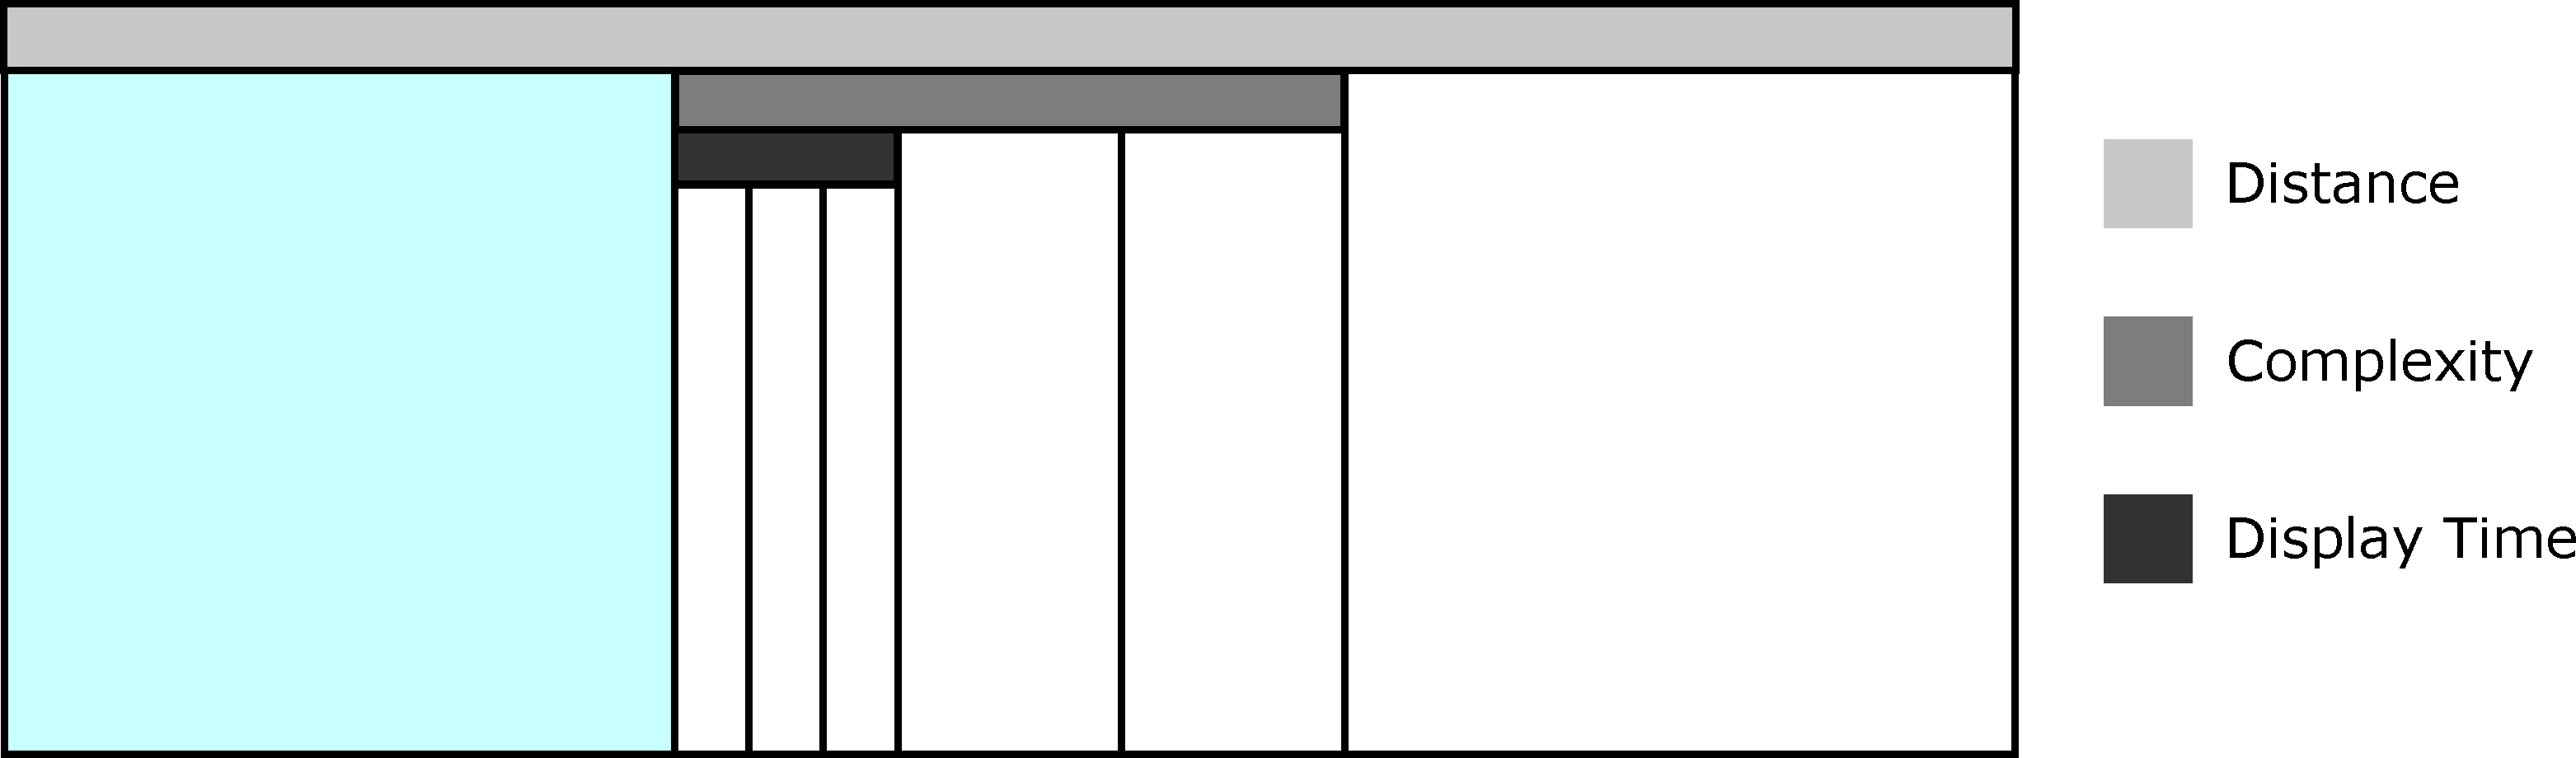
\includegraphics[width=110mm]{images/testCombination}
%		\caption{How tests will be combined in order to reduce the total number of tests.}
%		\label{testCombination}
%	\end{figure}


%[TODO Inledande text]


%Text Length - how much text can you fit on the Google Glass screen compared to smartphone? How many slides does a full slide on the smartphone take up on Google Glass?


%Speed - Compare speed between google glass and smartphone, from scanning the qr code till the slide view is ready


%recognizing the qr code - is there a difference between google glass and smartphone? Use different sizes of the qr code, as well different scaled versions. DIfferent complexity. Is there any difference in speed? Does Google Glass recognize them all?


%tap counter - how many taps to start compared to smartphone (widget vs simple app)


%user experience - do they prefer google glass or smartphone?


%background noise? How to test scientifically?






%\subsection{Text Length}
%Since the Google Glass display is small and limited in space the amount of text that may by displayed on screen is as a result also limited. As such one interesting test case is to see where the limit in text lies. The test consists of trying different text lengths and reaching a conclusion on how much text may be displayed. The test also includes using different characters as different characters allocates different amounts of space.

%\subsection{Image Size}
%Similar to text images are also limited to the screen size. However, in terms of images there is a slightly different issue compared to text. Images may be resized to fit the screen. Is there a point where and image is no longer usable as details in the original resolution can no longer be spotted in the resized version? The test consists of using images with different original resolutions and comparing how well details are shown.

%\subsection{Comparing Text and Images}
%todo

%\subsection{Download Speed}
%The download speed is important as users might not want to wait too long for the application to load in the instructions after having scanned the QR code. As such the download speed will be measured for different amounts of data sized, on both the smartphone application as well as the Google Glass application. 

%\subsection{Interaction Delay}
%todo

%\subsection{Background Noise}
%todo

%\subsection{Size of QR Code}
%todo

%\subsection{Complexity of QR Code}
%todo

%\subsection{``Tap Counter''}
%The ``tap counting test'' simply consists of counting the amount of taps a user must perform in order to reach specific destinations. For instance, how many taps must the user perform in order to start the application?

%\subsection{User Experience}
%todo

%\subsection{Multitasking}
%todo

%\subsection{Battery}
%todo

%\subsection{Connected to Mobile Device}
%todo

%\subsection{Overall Personal Opinions}
%todo